% aria_paper.tex
% Draft: Human--AI Collaboration in Producing an Undergraduate ERM Textbook
% Author: Martin F. Grace
% Draft generated with assistance from Composer (Cursor agent model), June 2026.
% =======================================================================
\documentclass[11pt,letterpaper]{article}

\usepackage[margin=1in]{geometry}
\usepackage{setspace}
% microtype omitted: MiKTeX font-expansion error on this system
\usepackage{amsmath,amssymb}
\usepackage{graphicx}
\usepackage{booktabs}
\usepackage{enumitem}
\usepackage{hyperref}
\usepackage{natbib}
\usepackage{tcolorbox}
\usepackage{textcomp}
\usepackage{tabularx}

\hypersetup{
  pdftitle={AI-Assisted Development of Comprehensive Course
Materials for Enterprise Risk Management},
  pdfauthor={Martin F. Grace},
  colorlinks=true,
  linkcolor=black,
  citecolor=black,
  urlcolor=black
}

\onehalfspacing
\hbadness=10001
\hfuzz=50pt

\newtcolorbox{draftnote}{
  colback=gray!8,
  colframe=gray!50,
  fonttitle=\bfseries,
  title={Draft metadata}
}

% --- PREAMBLE: just the title/author/date, nothing else ---
\title{\textbf{AI-Assisted Development of\\
Materials for Enterprise Risk Management}}

\author{Martin F. Grace%
  \thanks{Professor of Finance \& Hanson Family Chair; Faculty Director, 
  Vaughan Institute of Risk Management \& Insurance, Tippie College of 
  Business, University of Iowa. \texttt{mfgrace@uiowa.edu}.}%
}

\date{\small\textit{Draft prepared June 2026}}


\begin{document}
\maketitle
\thispagestyle{empty}

% --- Acknowledgment note ---
\begin{center}
\begin{minipage}{0.92\textwidth}
\small I thank the students who read drafts and asked questions; the Vaughan
Institute of Risk Management \& Insurance at the University of Iowa's Tippie
College of Business (``Go Hawks!'') for providing the test subjects---I mean,
students. A big round of thanks also goes to the several large language models
that never asked for summer teaching relief or to attend a ski conference in New
Hampshire. The remaining errors, eccentric jokes, and any sentences that sound
overwrought are, probabilistically, my responsibility.
\end{minipage}
\end{center}

\begin{draftnote}
\textbf{Model used for this draft.} This paper was drafted with the assistance of \textbf{Composer} (Cursor's agent model, June 2026). The textbook project described below relied primarily on Anthropic's Claude 4.6 Sonnet and Claude 5 Fable (via Cursor), with Perplexity used for case examples.
\end{draftnote}


% Add this where you want the figure to appear in your text:
\begin{figure}[htbp]
    \centering
    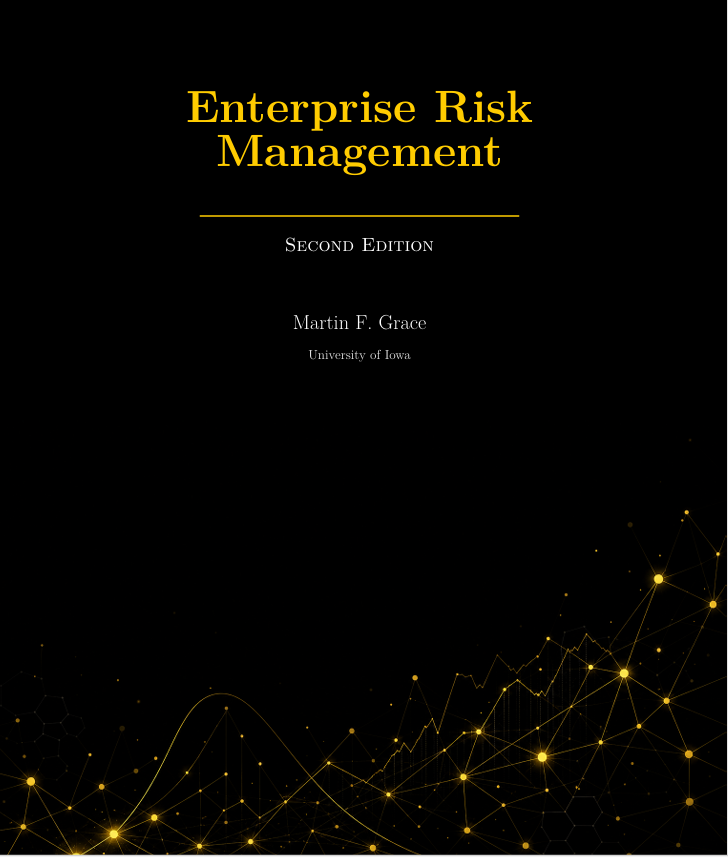
\includegraphics[width=0.9\textwidth]{figs/cover.PNG}
    \caption{Cover art, \textit{Enterprise Risk Management}, second edition.}
    \label{fig:coverart}
\end{figure}

\begin{abstract}
\noindent
This paper is an overview of how I ``wrote'' what I am calling the second edition of an undergraduate enterprise risk management (ERM) textbook. I ``wrote'' the textbook through sustained collaboration with large language models (LLMs). This project began with a full outline and a working draft that I piloted in class in the Spring of 2026. I then followed up with a structural overhaul, chapter-level rewrites aimed at engagement and pedagogical clarity, and the development of a unified production pipeline that produced a \LaTeX-typeset PDF file. I added opening cases, checked the numbers and math, and built the book as an integrated object with a text, cover, bibliography, index, and Beamer-style \LaTeX{} slides. Generative AI accelerated drafting and formatting, but I retained responsibility for the institutional nuances, economics, regulatory judgments, fact-checking, and the final prose. In what follows, I lay out that workflow, what worked and what did not, and what this might mean for academic authorship when the marginal cost of a ``reasonable first draft'' is close to zero. The lame jokes are mine, and the LLMs are not to blame.

\end{abstract}

% =============================================================================
% toc_only.tex — Complete table of contents for *Enterprise Risk Management*,
% Second Edition. All entries embedded; does not \input{} any other file.
%
% Requires a book-class document with hyperref (e.g., erm_textbook_style).
% Snapshot from integrated book build, June 2026.
%
% Usage — \input{toc_only.tex} after \begin{document} (book or article + hyperref).
% The heading is included in this file; no \chapter*{Table of Contents} needed.
% =============================================================================
\clearpage
\leavevmode\par
{\centering\normalfont\Large\bfseries Table of Contents\par}
\vspace{0.75em}

\begingroup
\footnotesize
\setlength{\parskip}{2pt}
\setcounter{tocdepth}{3}
\makeatletter
\let\oldaddvspace\addvspace
\renewcommand{\addvspace}[1]{}%
\@ifundefined{l@chapter}{%
  \def\l@chapter#1#2{\@dottedtocline{0}{0em}{2.5em}}%
}{}%
\hypersetup{linktocpage=true}%
\def\@pnumwidth{2.35em}
\def\@tocrmarg{3.0em}
\renewcommand*\l@section{\@dottedtocline{1}{0em}{5.25em}}
\renewcommand*\l@subsection{\@dottedtocline{2}{1.5em}{5.75em}}
\renewcommand*\l@subsubsection{\@dottedtocline{3}{3.25em}{6.25em}}
\renewcommand*\l@chapter[2]{%
  \ifnum \c@tocdepth >\m@ne
    \addpenalty{-\@highpenalty}%
    \vskip 0.75em \@plus\p@
    \setlength\@tempdima{2.0em}%
    \begingroup
      \parindent \z@ \rightskip \@pnumwidth
      \parfillskip -\@pnumwidth
      \leavevmode \bfseries
      \advance\leftskip\@tempdima
      \hskip -\leftskip
      #1\nobreak\hfil \nobreak\hb@xt@\@pnumwidth{\hss #2}\par
      \penalty\@highpenalty
    \endgroup
  \fi}
\makeatother

\contentsline {chapter}{Preface}{iii}{section*.2}%
\contentsline {chapter}{\numberline {1}Why Risk Management Matters}{1}{chapter.1}%
\contentsline {section}{\numberline {1.1}Introduction: The Paradox of Risk Management}{3}{section.1.1}%
\contentsline {section}{\numberline {1.2}The Benchmark: Risk Management Is Irrelevant in Perfect Markets}{4}{section.1.2}%
\contentsline {subsection}{\numberline {1.2.1}The Modigliani--Miller Propositions}{4}{subsection.1.2.1}%
\contentsline {subsection}{\numberline {1.2.2}The Capital Asset Pricing Model (CAPM)}{4}{subsection.1.2.2}%
\contentsline {subsection}{\numberline {1.2.3}Risk Management Irrelevance Under Perfect Markets}{5}{subsection.1.2.3}%
\contentsline {section}{\numberline {1.3}Assumptions Behind CAPM and MM Irrelevance}{5}{section.1.3}%
\contentsline {subsection}{\numberline {1.3.1}Detailed CAPM Assumptions}{6}{subsection.1.3.1}%
\contentsline {subsection}{\numberline {1.3.2}Modigliani--Miller Assumptions (Overlapping with CAPM)}{7}{subsection.1.3.2}%
\contentsline {subsection}{\numberline {1.3.3}What Irrelevance Means}{8}{subsection.1.3.3}%
\contentsline {section}{\numberline {1.4}Real-World Frictions That Make Risk Management Matter}{8}{section.1.4}%
\contentsline {subsection}{\numberline {1.4.1}Taxes and Tax Convexity}{8}{subsection.1.4.1}%
\contentsline {subsection}{\numberline {1.4.2}Costly Financial Distress and Bankruptcy}{9}{subsection.1.4.2}%
\contentsline {subsection}{\numberline {1.4.3}Investment Distortions and Underinvestment}{10}{subsection.1.4.3}%
\contentsline {subsection}{\numberline {1.4.4}Principal--Agent Problems and Managerial Incentives}{10}{subsection.1.4.4}%
\contentsline {subsection}{\numberline {1.4.5}Information Asymmetry and Signaling}{11}{subsection.1.4.5}%
\contentsline {subsection}{\numberline {1.4.6}Contracting and Stakeholder Relationships}{12}{subsection.1.4.6}%
\contentsline {subsection}{\numberline {1.4.7}Regulatory and Rating-Agency Constraints}{13}{subsection.1.4.7}%
\contentsline {section}{\numberline {1.5}The Cost of Risk and the Objective of Corporate Risk Management}{14}{section.1.5}%
\contentsline {subsection}{\numberline {1.5.1}Defining the Cost of Risk}{14}{subsection.1.5.1}%
\contentsline {subsection}{\numberline {1.5.2}The Objective of Corporate Risk Management}{14}{subsection.1.5.2}%
\contentsline {subsection}{\numberline {1.5.3}Risk Management as Core Corporate Finance}{15}{subsection.1.5.3}%
\contentsline {section}{\numberline {1.6}Roadmap for the Rest of the Book}{15}{section.1.6}%
\contentsline {section}{Key Takeaways}{16}{section.1.6}%
\contentsline {section}{References}{16}{section.1.6}%
\contentsline {chapter}{\numberline {2}Enterprise Risk Management: Evolution, Frameworks, and Institutional Context}{18}{chapter.2}%
\contentsline {section}{\numberline {2.1}The Evolution of Corporate Risk Management}{20}{section.2.1}%
\contentsline {subsection}{\numberline {2.1.1}From Insurance to Integration}{20}{subsection.2.1.1}%
\contentsline {subsection}{\numberline {2.1.2}The Sarbanes-Oxley Inflection}{21}{subsection.2.1.2}%
\contentsline {section}{\numberline {2.2}The Two Dominant Frameworks}{21}{section.2.2}%
\contentsline {subsection}{\numberline {2.2.1}The COSO ERM Framework}{21}{subsection.2.2.1}%
\contentsline {subsection}{\numberline {2.2.2}The ISO~31000 Standard}{23}{subsection.2.2.2}%
\contentsline {subsection}{\numberline {2.2.3}COSO and ISO~31000: Where They Differ and Where They Converge}{23}{subsection.2.2.3}%
\contentsline {section}{\numberline {2.3}The Institutional Landscape}{24}{section.2.3}%
\contentsline {subsection}{\numberline {2.3.1}Financial Services: Regulation as the Driver}{24}{subsection.2.3.1}%
\contentsline {subsection}{\numberline {2.3.2}Non-Financial Corporations: Voluntary but Not Casual}{25}{subsection.2.3.2}%
\contentsline {section}{\numberline {2.4}Implementing ERM: What It Actually Takes}{25}{section.2.4}%
\contentsline {section}{Key Takeaways}{26}{section.2.4}%
\contentsline {section}{References}{27}{section.2.4}%
\contentsline {chapter}{\numberline {3}Risk Identification: Categorizing and Discovering Enterprise Risks}{28}{chapter.3}%
\contentsline {section}{\numberline {3.1}The Four Quadrants of Risk}{30}{section.3.1}%
\contentsline {subsection}{\numberline {3.1.1}Hazard Risks}{30}{subsection.3.1.1}%
\contentsline {subsection}{\numberline {3.1.2}Financial Risks}{31}{subsection.3.1.2}%
\contentsline {subsection}{\numberline {3.1.3}Operational Risks}{32}{subsection.3.1.3}%
\contentsline {subsubsection}{Business Interruption: An Operational Risk, Not a Financial Risk}{33}{subsubsection*.5}%
\contentsline {subsection}{\numberline {3.1.4}Strategic Risks}{34}{subsection.3.1.4}%
\contentsline {subsection}{\numberline {3.1.5}Risk Interdependencies and the Limits of Categorization}{34}{subsection.3.1.5}%
\contentsline {section}{\numberline {3.2}Sources of Risk and Risk Identification Methodologies}{35}{section.3.2}%
\contentsline {subsection}{\numberline {3.2.1}Internal Sources of Risk Information}{35}{subsection.3.2.1}%
\contentsline {subsection}{\numberline {3.2.2}External Sources of Risk Information}{36}{subsection.3.2.2}%
\contentsline {subsection}{\numberline {3.2.3}Risk Identification Techniques}{36}{subsection.3.2.3}%
\contentsline {subsection}{\numberline {3.2.4}Integrating Risk Identification into Organizational Processes}{37}{subsection.3.2.4}%
\contentsline {section}{\numberline {3.3}The SEC Form~10-K Risk Factors Disclosure}{37}{section.3.3}%
\contentsline {subsection}{\numberline {3.3.1}Regulatory Background and Requirements}{37}{subsection.3.3.1}%
\contentsline {subsection}{\numberline {3.3.2}Structure and Content of Risk Factors Disclosures}{38}{subsection.3.3.2}%
\contentsline {subsection}{\numberline {3.3.3}Using Risk Factors for Risk Identification and Analysis}{39}{subsection.3.3.3}%
\contentsline {subsection}{\numberline {3.3.4}Limitations of Risk Factors Disclosures}{39}{subsection.3.3.4}%
\contentsline {section}{Key Takeaways}{40}{subsection.3.3.4}%
\contentsline {section}{References}{40}{subsection.3.3.4}%
\contentsline {chapter}{\numberline {4}Risk Quantification and Qualification}{42}{chapter.4}%
\contentsline {section}{\numberline {4.1}Why Quantify and Qualify Risk?}{46}{section.4.1}%
\contentsline {subsection}{\numberline {4.1.1}The Limitations of Intuition and Informal Assessment}{46}{subsection.4.1.1}%
\contentsline {subsection}{\numberline {4.1.2}The Value of Quantitative Risk Measurement}{47}{subsection.4.1.2}%
\contentsline {subsection}{\numberline {4.1.3}Quantification Beyond Finance: Non-Financial Companies}{48}{subsection.4.1.3}%
\contentsline {subsection}{\numberline {4.1.4}The Continuing Role of Qualitative Assessment}{49}{subsection.4.1.4}%
\contentsline {section}{\numberline {4.2}Basic Statistical Tools for Risk Measurement}{49}{section.4.2}%
\contentsline {subsection}{\numberline {4.2.1}Frequency, Severity, and Expected Loss}{49}{subsection.4.2.1}%
\contentsline {subsection}{\numberline {4.2.2}Descriptive Statistics: Mean, Median, Variance, and Standard Deviation}{50}{subsection.4.2.2}%
\contentsline {subsection}{\numberline {4.2.3}Correlation and Risk Aggregation}{51}{subsection.4.2.3}%
\contentsline {subsection}{\numberline {4.2.4}Probability Distributions and Loss Distributions}{51}{subsection.4.2.4}%
\contentsline {section}{\numberline {4.3}Case Study: Quantifying Risk at Midtown Outfitters (Retailer)}{52}{section.4.3}%
\contentsline {subsection}{\numberline {4.3.1}Company Background and Risk Landscape}{52}{subsection.4.3.1}%
\contentsline {subsection}{\numberline {4.3.2}Data Collection and Organization}{52}{subsection.4.3.2}%
\contentsline {subsection}{\numberline {4.3.3}Quantifying Slip-and-Fall Incidents}{53}{subsection.4.3.3}%
\contentsline {subsection}{\numberline {4.3.4}Quantifying Inventory Shrinkage}{53}{subsection.4.3.4}%
\contentsline {subsection}{\numberline {4.3.5}Quantifying Property Damage}{54}{subsection.4.3.5}%
\contentsline {subsection}{\numberline {4.3.6}Risk Matrix and Prioritization}{54}{subsection.4.3.6}%
\contentsline {subsection}{\numberline {4.3.7}Management Interpretation and Decisions}{54}{subsection.4.3.7}%
\contentsline {section}{\numberline {4.4}Case Study: Quantifying Risk at Precision Parts Inc.\ (Manufacturer)}{55}{section.4.4}%
\contentsline {subsection}{\numberline {4.4.1}Company Background}{55}{subsection.4.4.1}%
\contentsline {subsection}{\numberline {4.4.2}Quantifying Equipment Breakdown and Downtime}{55}{subsection.4.4.2}%
\contentsline {subsection}{\numberline {4.4.3}Quantifying Product Defects and Warranty Claims}{56}{subsection.4.4.3}%
\contentsline {subsection}{\numberline {4.4.4}Quantifying Workplace Injury Risk}{56}{subsection.4.4.4}%
\contentsline {subsection}{\numberline {4.4.5}Risk Correlations and Compounding Effects}{56}{subsection.4.4.5}%
\contentsline {subsection}{\numberline {4.4.6}Qualitative Risk Assessment for Manufacturing}{57}{subsection.4.4.6}%
\contentsline {section}{\numberline {4.5}Loss Distributions and Skewness}{57}{section.4.5}%
\contentsline {subsection}{\numberline {4.5.1}The Normal Distribution}{57}{subsection.4.5.1}%
\contentsline {subsection}{\numberline {4.5.2}Right-Skewed Distributions and Tail Risk}{57}{subsection.4.5.2}%
\contentsline {subsection}{\numberline {4.5.3}Why Skewness Matters for Risk Management}{58}{subsection.4.5.3}%
\contentsline {subsection}{\numberline {4.5.4}Measuring and Describing Skewness}{58}{subsection.4.5.4}%
\contentsline {section}{\numberline {4.6}Excel-Based Workers' Compensation Case: Estimating Value at Risk}{59}{section.4.6}%
\contentsline {subsection}{\numberline {4.6.1}Company Background: Northland Manufacturing}{59}{subsection.4.6.1}%
\contentsline {subsection}{\numberline {4.6.2}Data Description}{59}{subsection.4.6.2}%
\contentsline {subsection}{\numberline {4.6.3}Step-by-Step Excel Analysis}{59}{subsection.4.6.3}%
\contentsline {subsection}{\numberline {4.6.4}Calculating Value at Risk}{60}{subsection.4.6.4}%
\contentsline {subsection}{\numberline {4.6.5}Interpreting and Using VaR}{61}{subsection.4.6.5}%
\contentsline {section}{\numberline {4.7}Value at Risk: Usefulness and Limitations}{61}{section.4.7}%
\contentsline {subsection}{\numberline {4.7.1}Why VaR Is Appealing}{61}{subsection.4.7.1}%
\contentsline {subsection}{\numberline {4.7.2}Limitations of VaR}{61}{subsection.4.7.2}%
\contentsline {subsection}{\numberline {4.7.3}Complementary Risk Measures}{62}{subsection.4.7.3}%
\contentsline {subsection}{\numberline {4.7.4}Integrating VaR into Risk Management}{62}{subsection.4.7.4}%
\contentsline {section}{\numberline {4.8}Limits of Quantitative Measures and the Role of Qualitative Assessment}{63}{section.4.8}%
\contentsline {subsection}{\numberline {4.8.1}When Quantification Is Most Valuable}{63}{subsection.4.8.1}%
\contentsline {subsection}{\numberline {4.8.2}When Qualitative Assessment Is Essential}{63}{subsection.4.8.2}%
\contentsline {subsection}{\numberline {4.8.3}Integrating Quantitative and Qualitative Assessment}{63}{subsection.4.8.3}%
\contentsline {subsection}{\numberline {4.8.4}The Art and Science of Risk Assessment}{64}{subsection.4.8.4}%
\contentsline {section}{Key Takeaways}{64}{subsection.4.8.4}%
\contentsline {section}{Key Terms}{65}{subsection.4.8.4}%
\contentsline {section}{Short-Answer Questions}{66}{subsection.4.8.4}%
\contentsline {section}{Discussion Questions}{66}{Item.45}%
\contentsline {section}{Mini-Case: Workers' Compensation Risk Analysis: Northland Manufacturing}{67}{Item.54}%
\contentsline {section}{References}{68}{Item.54}%
\contentsline {chapter}{\numberline {5}Risk Appetite and the ERM Process}{69}{chapter.5}%
\contentsline {section}{\numberline {5.1}Why Risk Appetite Matters}{72}{section.5.1}%
\contentsline {subsection}{\numberline {5.1.1}Risk Appetite as Strategic Choice}{72}{subsection.5.1.1}%
\contentsline {subsection}{\numberline {5.1.2}The Consequences of Unclear Risk Appetite}{73}{subsection.5.1.2}%
\contentsline {subsection}{\numberline {5.1.3}Risk Appetite and Value Creation}{73}{subsection.5.1.3}%
\contentsline {section}{\numberline {5.2}Defining Risk Appetite and Related Concepts}{74}{section.5.2}%
\contentsline {subsection}{\numberline {5.2.1}Risk Appetite: Core Definition}{74}{subsection.5.2.1}%
\contentsline {subsection}{\numberline {5.2.2}Risk Capacity: The Maximum Boundary}{74}{subsection.5.2.2}%
\contentsline {subsection}{\numberline {5.2.3}Risk Tolerance: Acceptable Variation Around Objectives}{74}{subsection.5.2.3}%
\contentsline {subsection}{\numberline {5.2.4}Risk Limits: Operational Constraints}{75}{subsection.5.2.4}%
\contentsline {subsection}{\numberline {5.2.5}The Hierarchy: Capacity, Appetite, Tolerance, and Limits}{75}{subsection.5.2.5}%
\contentsline {section}{\numberline {5.3}Risk Appetite in the ERM Cycle}{76}{section.5.3}%
\contentsline {subsection}{\numberline {5.3.1}The Sequence in Theory and in Practice}{76}{subsection.5.3.1}%
\contentsline {subsection}{\numberline {5.3.2}The Mature ERM Cycle: Appetite as Starting Point}{76}{subsection.5.3.2}%
\contentsline {subsection}{\numberline {5.3.3}Risk Appetite and Risk Identification}{77}{subsection.5.3.3}%
\contentsline {subsection}{\numberline {5.3.4}Risk Appetite in Risk Assessment}{77}{subsection.5.3.4}%
\contentsline {subsection}{\numberline {5.3.5}Risk Appetite Driving Risk Response}{77}{subsection.5.3.5}%
\contentsline {subsection}{\numberline {5.3.6}Risk Appetite in Monitoring and Review}{78}{subsection.5.3.6}%
\contentsline {section}{\numberline {5.4}Translating Risk Appetite into Limits, Tolerances, and Metrics}{78}{section.5.4}%
\contentsline {subsection}{\numberline {5.4.1}The Cascading Process}{78}{subsection.5.4.1}%
\contentsline {subsection}{\numberline {5.4.2}Characteristics of Effective Limits}{79}{subsection.5.4.2}%
\contentsline {subsection}{\numberline {5.4.3}Key Risk Indicators}{79}{subsection.5.4.3}%
\contentsline {section}{\numberline {5.5}Qualitative Articulation of Risk Appetite}{79}{section.5.5}%
\contentsline {subsection}{\numberline {5.5.1}The Role of Narrative Risk Appetite Statements}{79}{subsection.5.5.1}%
\contentsline {subsection}{\numberline {5.5.2}Components of Effective Risk Appetite Statements}{79}{subsection.5.5.2}%
\contentsline {subsection}{\numberline {5.5.3}Visual Tools: Matrices and Heat Maps}{80}{subsection.5.5.3}%
\contentsline {section}{\numberline {5.6}Quantitative Articulation of Risk Appetite}{80}{section.5.6}%
\contentsline {subsection}{\numberline {5.6.1}Linking Risk Appetite to Financial Metrics}{80}{subsection.5.6.1}%
\contentsline {subsection}{\numberline {5.6.2}Value at Risk as a Risk Appetite Metric}{81}{subsection.5.6.2}%
\contentsline {subsection}{\numberline {5.6.3}Economic Capital and Capital Adequacy}{81}{subsection.5.6.3}%
\contentsline {subsection}{\numberline {5.6.4}Concentration Limits}{81}{subsection.5.6.4}%
\contentsline {subsection}{\numberline {5.6.5}Scenario Analysis and Reverse Stress Testing}{82}{subsection.5.6.5}%
\contentsline {section}{\numberline {5.7}Risk Appetite for Different Types of Firms}{82}{section.5.7}%
\contentsline {subsection}{\numberline {5.7.1}InnovateTech: High-Growth Technology Company}{82}{subsection.5.7.1}%
\contentsline {subsection}{\numberline {5.7.2}Midwest Property \& Casualty: Established Regional Insurer}{83}{subsection.5.7.2}%
\contentsline {subsection}{\numberline {5.7.3}PowerGrid: Regulated Electric Utility}{83}{subsection.5.7.3}%
\contentsline {section}{\numberline {5.8}Governance, Culture, and Communication}{84}{section.5.8}%
\contentsline {subsection}{\numberline {5.8.1}Board and Senior Management Roles}{84}{subsection.5.8.1}%
\contentsline {subsection}{\numberline {5.8.2}Incentives and Compensation Alignment}{84}{subsection.5.8.2}%
\contentsline {subsection}{\numberline {5.8.3}Risk Culture}{85}{subsection.5.8.3}%
\contentsline {section}{\numberline {5.9}Common Pitfalls and Failures in Risk Appetite Frameworks}{85}{section.5.9}%
\contentsline {subsection}{\numberline {5.9.1}Case Example: Risk Appetite in the 2008 Financial Crisis}{86}{subsection.5.9.1}%
\contentsline {section}{Key Takeaways}{86}{subsection.5.9.1}%
\contentsline {section}{Key Terms}{87}{subsection.5.9.1}%
\contentsline {section}{Discussion Questions}{88}{subsection.5.9.1}%
\contentsline {section}{Mini-Case: Developing Risk Appetite for TechManufacture Inc.}{89}{Item.72}%
\contentsline {section}{References}{90}{Item.77}%
\contentsline {chapter}{\numberline {6}Examining the Firm's Risk Portfolio}{91}{chapter.6}%
\contentsline {section}{\numberline {6.1}From Individual Risks to Portfolio Perspective}{93}{section.6.1}%
\contentsline {subsection}{\numberline {6.1.1}The Limits of Individual Risk Analysis}{94}{subsection.6.1.1}%
\contentsline {subsection}{\numberline {6.1.2}The Portfolio Metaphor from Finance}{94}{subsection.6.1.2}%
\contentsline {subsection}{\numberline {6.1.3}What Changes with Portfolio Thinking}{95}{subsection.6.1.3}%
\contentsline {section}{\numberline {6.2}What Is a Risk Portfolio?}{95}{section.6.2}%
\contentsline {subsection}{\numberline {6.2.1}Defining the Risk Portfolio}{95}{subsection.6.2.1}%
\contentsline {subsection}{\numberline {6.2.2}Risk Categories in the Portfolio}{95}{subsection.6.2.2}%
\contentsline {subsection}{\numberline {6.2.3}Materiality: What Belongs in the Portfolio?}{96}{subsection.6.2.3}%
\contentsline {section}{\numberline {6.3}Why Risk Aggregation Matters for Enterprise Decision-Making}{96}{section.6.3}%
\contentsline {subsection}{\numberline {6.3.1}Economic Capital and Capital Allocation}{96}{subsection.6.3.1}%
\contentsline {subsection}{\numberline {6.3.2}Risk Appetite Compliance}{97}{subsection.6.3.2}%
\contentsline {subsection}{\numberline {6.3.3}Strategic Decisions and Portfolio Optimization}{97}{subsection.6.3.3}%
\contentsline {section}{\numberline {6.4}Mapping and Inventorying the Firm's Risk Portfolio}{98}{section.6.4}%
\contentsline {subsection}{\numberline {6.4.1}Building the Risk Register}{98}{subsection.6.4.1}%
\contentsline {subsection}{\numberline {6.4.2}Risk Register Example}{98}{subsection.6.4.2}%
\contentsline {subsection}{\numberline {6.4.3}The Risk Mapping Process}{100}{subsection.6.4.3}%
\contentsline {subsection}{\numberline {6.4.4}Common Pitfalls in Risk Inventories}{100}{subsection.6.4.4}%
\contentsline {section}{\numberline {6.5}Understanding Risk Correlations and Dependencies}{100}{section.6.5}%
\contentsline {subsection}{\numberline {6.5.1}Correlation: Definition and Interpretation}{100}{subsection.6.5.1}%
\contentsline {subsection}{\numberline {6.5.2}Why Correlation Affects Portfolio Risk}{101}{subsection.6.5.2}%
\contentsline {subsection}{\numberline {6.5.3}Constructing a Correlation Matrix}{101}{subsection.6.5.3}%
\contentsline {subsection}{\numberline {6.5.4}Estimating Correlations in Practice}{102}{subsection.6.5.4}%
\contentsline {subsection}{\numberline {6.5.5}Tail Dependence and Correlation Breakdown}{102}{subsection.6.5.5}%
\contentsline {section}{\numberline {6.6}Quantitative Risk Aggregation Techniques}{103}{section.6.6}%
\contentsline {subsection}{\numberline {6.6.1}Method 1: Simple Summation (Conservative Upper Bound)}{103}{subsection.6.6.1}%
\contentsline {subsection}{\numberline {6.6.2}Method 2: Variance-Covariance Aggregation}{103}{subsection.6.6.2}%
\contentsline {subsection}{\numberline {6.6.3}Method 3: Monte Carlo Simulation}{104}{subsection.6.6.3}%
\contentsline {subsection}{\numberline {6.6.4}Method 4: Copula-Based Aggregation (Conceptual Overview)}{105}{subsection.6.6.4}%
\contentsline {section}{\numberline {6.7}Building the Aggregate Loss Distribution}{106}{section.6.7}%
\contentsline {subsection}{\numberline {6.7.1}What the Aggregate Loss Distribution Shows}{106}{subsection.6.7.1}%
\contentsline {subsection}{\numberline {6.7.2}Comparing Individual and Aggregate Distributions}{106}{subsection.6.7.2}%
\contentsline {subsection}{\numberline {6.7.3}Key Metrics from the Aggregate Distribution}{106}{subsection.6.7.3}%
\contentsline {subsection}{\numberline {6.7.4}Interpreting the Aggregate Distribution for Management}{107}{subsection.6.7.4}%
\contentsline {section}{\numberline {6.8}Diversification Benefits and Portfolio Risk Reduction}{107}{section.6.8}%
\contentsline {subsection}{\numberline {6.8.1}Quantifying Diversification Benefit}{107}{subsection.6.8.1}%
\contentsline {subsection}{\numberline {6.8.2}Factors Affecting Diversification}{107}{subsection.6.8.2}%
\contentsline {subsection}{\numberline {6.8.3}Strategic Implications of Diversification}{108}{subsection.6.8.3}%
\contentsline {subsection}{\numberline {6.8.4}Limits of Diversification}{108}{subsection.6.8.4}%
\contentsline {section}{\numberline {6.9}Stress Testing and Scenario Analysis for the Total Portfolio}{108}{section.6.9}%
\contentsline {subsection}{\numberline {6.9.1}Why Stress Test the Portfolio?}{109}{subsection.6.9.1}%
\contentsline {subsection}{\numberline {6.9.2}Designing Portfolio Stress Tests}{109}{subsection.6.9.2}%
\contentsline {subsection}{\numberline {6.9.3}Example: Portfolio Stress Test}{109}{subsection.6.9.3}%
\contentsline {subsection}{\numberline {6.9.4}Integrating Stress Tests into Governance}{110}{subsection.6.9.4}%
\contentsline {section}{\numberline {6.10}Integrating Risk Portfolio Analysis with Risk Appetite}{110}{section.6.10}%
\contentsline {subsection}{\numberline {6.10.1}Portfolio Metrics as Risk Appetite Measures}{110}{subsection.6.10.1}%
\contentsline {subsection}{\numberline {6.10.2}New Risk Evaluation: Incremental Portfolio Impact}{111}{subsection.6.10.2}%
\contentsline {subsection}{\numberline {6.10.3}Capital Allocation Using Portfolio Analysis}{111}{subsection.6.10.3}%
\contentsline {section}{\numberline {6.11}Practical Implementation: Tools and Organizational Challenges}{112}{section.6.11}%
\contentsline {subsection}{\numberline {6.11.1}Data Challenges}{112}{subsection.6.11.1}%
\contentsline {subsection}{\numberline {6.11.2}Model Risk and Validation}{112}{subsection.6.11.2}%
\contentsline {subsection}{\numberline {6.11.3}Organizational and Cultural Challenges}{112}{subsection.6.11.3}%
\contentsline {subsection}{\numberline {6.11.4}Technology and Tools}{113}{subsection.6.11.4}%
\contentsline {section}{\numberline {6.12}Case Study: Constructing a Risk Portfolio for Global Manufacturing Co.}{113}{section.6.12}%
\contentsline {subsection}{\numberline {6.12.1}Company Background}{113}{subsection.6.12.1}%
\contentsline {subsection}{\numberline {6.12.2}Risk Inventory and Assessment}{114}{subsection.6.12.2}%
\contentsline {subsection}{\numberline {6.12.3}Correlation Assessment}{114}{subsection.6.12.3}%
\contentsline {subsection}{\numberline {6.12.4}Portfolio Aggregation}{114}{subsection.6.12.4}%
\contentsline {subsection}{\numberline {6.12.5}Monte Carlo Validation}{115}{subsection.6.12.5}%
\contentsline {subsection}{\numberline {6.12.6}Stress Testing}{115}{subsection.6.12.6}%
\contentsline {subsection}{\numberline {6.12.7}Management Actions and Portfolio Optimization}{117}{subsection.6.12.7}%
\contentsline {section}{Key Takeaways}{117}{subsection.6.12.7}%
\contentsline {section}{Key Terms}{118}{subsection.6.12.7}%
\contentsline {section}{Discussion Questions}{120}{subsection.6.12.7}%
\contentsline {section}{Mini-Case: Portfolio Risk Exercise --- TechRetail Corp}{121}{Item.115}%
\contentsline {section}{Advanced Challenge: Monte Carlo Portfolio Simulation}{122}{Item.127}%
\contentsline {section}{References}{123}{Item.132}%
\contentsline {chapter}{\numberline {7}Loss Control and Risk Reduction}{124}{chapter.7}%
\contentsline {section}{\numberline {7.1}From Risk Identification to Risk Reduction}{127}{section.7.1}%
\contentsline {subsection}{\numberline {7.1.1}The Loss Control Imperative}{127}{subsection.7.1.1}%
\contentsline {subsection}{\numberline {7.1.2}Loss Control in the ERM Framework}{127}{subsection.7.1.2}%
\contentsline {section}{\numberline {7.2}The Economics of Loss Control}{128}{section.7.2}%
\contentsline {subsection}{\numberline {7.2.1}The Total Cost of Risk Framework}{128}{subsection.7.2.1}%
\contentsline {subsection}{\numberline {7.2.2}Loss Control Return on Investment}{129}{subsection.7.2.2}%
\contentsline {subsection}{\numberline {7.2.3}Diminishing Returns and Optimal Investment}{129}{subsection.7.2.3}%
\contentsline {section}{\numberline {7.3}Frequency Reduction Techniques}{130}{section.7.3}%
\contentsline {subsection}{\numberline {7.3.1}The Logic of Frequency Control}{130}{subsection.7.3.1}%
\contentsline {subsection}{\numberline {7.3.2}Engineering-Based Frequency Reduction}{130}{subsection.7.3.2}%
\contentsline {subsection}{\numberline {7.3.3}Procedural and Administrative Frequency Reduction}{131}{subsection.7.3.3}%
\contentsline {subsection}{\numberline {7.3.4}Training and Competency Development}{131}{subsection.7.3.4}%
\contentsline {section}{\numberline {7.4}Severity Control Strategies}{132}{section.7.4}%
\contentsline {subsection}{\numberline {7.4.1}The Logic of Severity Control}{132}{subsection.7.4.1}%
\contentsline {subsection}{\numberline {7.4.2}Property Damage Severity Control}{132}{subsection.7.4.2}%
\contentsline {subsection}{\numberline {7.4.3}Injury Severity Control}{133}{subsection.7.4.3}%
\contentsline {subsection}{\numberline {7.4.4}Business Interruption Severity Control}{133}{subsection.7.4.4}%
\contentsline {section}{\numberline {7.5}Engineering Controls and Physical Safeguards}{134}{section.7.5}%
\contentsline {subsection}{\numberline {7.5.1}Machine Guarding and Point-of-Operation Protection}{134}{subsection.7.5.1}%
\contentsline {subsection}{\numberline {7.5.2}Electrical Safety Controls}{135}{subsection.7.5.2}%
\contentsline {subsection}{\numberline {7.5.3}Fall Protection Systems}{135}{subsection.7.5.3}%
\contentsline {section}{\numberline {7.6}Administrative Controls and Behavioral Interventions}{136}{section.7.6}%
\contentsline {subsection}{\numberline {7.6.1}Safety Culture and Leadership Engagement}{136}{subsection.7.6.1}%
\contentsline {subsection}{\numberline {7.6.2}Behavioral Safety Programs}{136}{subsection.7.6.2}%
\contentsline {subsection}{\numberline {7.6.3}Leading and Lagging Indicators}{137}{subsection.7.6.3}%
\contentsline {section}{\numberline {7.7}The Hierarchy of Controls Framework}{138}{section.7.7}%
\contentsline {subsection}{\numberline {7.7.1}NIOSH Hierarchy of Controls}{138}{subsection.7.7.1}%
\contentsline {subsection}{\numberline {7.7.2}Applying the Hierarchy in Practice}{139}{subsection.7.7.2}%
\contentsline {subsection}{\numberline {7.7.3}Economic Considerations in Hierarchy Application}{139}{subsection.7.7.3}%
\contentsline {section}{\numberline {7.8}Loss Control in Different Industries}{140}{section.7.8}%
\contentsline {subsection}{\numberline {7.8.1}Manufacturing: Machine Guarding ROI}{140}{subsection.7.8.1}%
\contentsline {subsection}{\numberline {7.8.2}Retail: Slip-and-Fall Prevention}{141}{subsection.7.8.2}%
\contentsline {subsection}{\numberline {7.8.3}Construction: Fall Protection Systems}{142}{subsection.7.8.3}%
\contentsline {subsection}{\numberline {7.8.4}Healthcare: Workplace Violence Prevention}{144}{subsection.7.8.4}%
\contentsline {section}{\numberline {7.9}Measuring Loss Control Effectiveness}{145}{section.7.9}%
\contentsline {subsection}{\numberline {7.9.1}Standard Safety Metrics}{145}{subsection.7.9.1}%
\contentsline {subsection}{\numberline {7.9.2}Leading Indicators for Proactive Management}{146}{subsection.7.9.2}%
\contentsline {subsection}{\numberline {7.9.3}Benchmarking Against Industry Standards}{147}{subsection.7.9.3}%
\contentsline {section}{\numberline {7.10}Risk Financing vs.\ Risk Reduction Tradeoffs}{148}{section.7.10}%
\contentsline {subsection}{\numberline {7.10.1}The Total Cost of Risk Optimization}{148}{subsection.7.10.1}%
\contentsline {subsection}{\numberline {7.10.2}Practical Application: Deductible and Loss Control Interaction}{148}{subsection.7.10.2}%
\contentsline {subsection}{\numberline {7.10.3}Self-Insurance and Captive Insurance Considerations}{149}{subsection.7.10.3}%
\contentsline {section}{\numberline {7.11}Occupational Safety and Workers' Compensation Case Study}{150}{section.7.11}%
\contentsline {subsection}{\numberline {7.11.1}Riverside Metal Products: Baseline Risk Profile}{150}{subsection.7.11.1}%
\contentsline {subsection}{\numberline {7.11.2}Loss Control Interventions and Costs}{150}{subsection.7.11.2}%
\contentsline {subsection}{\numberline {7.11.3}Post-Control Results}{151}{subsection.7.11.3}%
\contentsline {subsection}{\numberline {7.11.4}Financial Analysis}{151}{subsection.7.11.4}%
\contentsline {section}{Key Takeaways}{152}{Item.144}%
\contentsline {section}{Key Terms}{153}{Item.144}%
\contentsline {section}{Discussion Questions}{155}{Item.144}%
\contentsline {section}{Mini-Case: Loss Control Program Design Assignment}{156}{Item.159}%
\contentsline {section}{References}{159}{Item.164}%
\contentsline {section}{Appendix 7A: The Economics and Finance of Loss Control Investment Decisions}{160}{Item.164}%
\contentsline {section}{\numberline {7A.1}Loss Control as Capital Investment}{160}{section.appendix7A.1}%
\contentsline {section}{\numberline {7A.2}The Multi-Period Discounted Cash Flow Model}{160}{section.appendix7A.2}%
\contentsline {subsection}{\numberline {7A.2.1}Baseline: No Loss Control}{160}{subsection.appendix7A.2.1}%
\contentsline {subsection}{\numberline {7A.2.2}Alternative: Implement Loss Control}{161}{subsection.appendix7A.2.2}%
\contentsline {subsection}{\numberline {7A.2.3}Net Present Value Decision Rule}{161}{subsection.appendix7A.2.3}%
\contentsline {subsection}{\numberline {7A.2.4}Relationship to the Simplified Model}{161}{subsection.appendix7A.2.4}%
\contentsline {section}{\numberline {7A.3}Selecting the Discount Rate}{161}{section.appendix7A.3}%
\contentsline {section}{\numberline {7A.4}Tax Effects and After-Tax Analysis}{162}{section.appendix7A.4}%
\contentsline {subsection}{\numberline {7A.4.1}Tax Treatment of Loss Control Costs}{162}{subsection.appendix7A.4.1}%
\contentsline {subsection}{\numberline {7A.4.2}Tax Treatment of Loss Reductions}{162}{subsection.appendix7A.4.2}%
\contentsline {subsection}{\numberline {7A.4.3}After-Tax NPV}{162}{subsection.appendix7A.4.3}%
\contentsline {section}{\numberline {7A.5}Insurance Premium Effects and EMR Dynamics}{163}{section.appendix7A.5}%
\contentsline {subsection}{\numberline {7A.5.1}Workers' Compensation Experience Rating}{163}{subsection.appendix7A.5.1}%
\contentsline {subsection}{\numberline {7A.5.2}Other Lines and the Complete Formula}{164}{subsection.appendix7A.5.2}%
\contentsline {section}{\numberline {7A.6}Indirect Costs, Unmeasured Benefits, and Tail Risk}{164}{section.appendix7A.6}%
\contentsline {subsection}{\numberline {7A.6.1}The Iceberg Model of Loss Costs}{164}{subsection.appendix7A.6.1}%
\contentsline {subsection}{\numberline {7A.6.2}Beyond Expected Value: Tail Risk and Financial Distress}{165}{subsection.appendix7A.6.2}%
\contentsline {section}{\numberline {7A.7}Real Options and Investment Timing}{165}{section.appendix7A.7}%
\contentsline {subsection}{\numberline {7A.7.1}The Option to Defer}{165}{subsection.appendix7A.7.1}%
\contentsline {subsection}{\numberline {7A.7.2}The Options to Expand and Abandon}{166}{subsection.appendix7A.7.2}%
\contentsline {section}{\numberline {7A.8}Portfolio Effects and Economic Capital}{166}{section.appendix7A.8}%
\contentsline {subsection}{\numberline {7A.8.1}Loss Control in the Risk Portfolio}{166}{subsection.appendix7A.8.1}%
\contentsline {subsection}{\numberline {7A.8.2}Capital Allocation and Risk Appetite}{166}{subsection.appendix7A.8.2}%
\contentsline {section}{\numberline {7A.9}Complete Numerical Example: Mercer Tool \& Stamping Revisited}{167}{section.appendix7A.9}%
\contentsline {section}{\numberline {7A.10}Notation Summary}{168}{section.appendix7A.10}%
\contentsline {section}{Appendix References}{168}{table.caption.18}%
\contentsline {chapter}{\numberline {8}Risk Finance and Alternative Risk Transfer}{170}{chapter.8}%
\contentsline {section}{\numberline {8.1}Risk Financing Follows Risk Control}{173}{section.8.1}%
\contentsline {subsection}{\numberline {8.1.1}The ERM Sequence: From Identification to Financing}{173}{subsection.8.1.1}%
\contentsline {subsection}{\numberline {8.1.2}The Risk Financing Decision Framework}{174}{subsection.8.1.2}%
\contentsline {subsection}{\numberline {8.1.3}Risk Financing and Organizational Value Creation}{174}{subsection.8.1.3}%
\contentsline {section}{\numberline {8.2}The Risk Financing Spectrum}{175}{section.8.2}%
\contentsline {subsection}{\numberline {8.2.1}The Continuum from Retention to Transfer}{175}{subsection.8.2.1}%
\contentsline {subsection}{\numberline {8.2.2}The Cost--Volatility Tradeoff}{176}{subsection.8.2.2}%
\contentsline {subsection}{\numberline {8.2.3}Factors Influencing Position on the Spectrum}{177}{subsection.8.2.3}%
\contentsline {section}{\numberline {8.3}Retention versus Transfer: The Core Decision}{177}{section.8.3}%
\contentsline {subsection}{\numberline {8.3.1}The Fundamental Cost Comparison}{177}{subsection.8.3.1}%
\contentsline {subsection}{\numberline {8.3.2}The Optimal Retention Level}{178}{subsection.8.3.2}%
\contentsline {subsection}{\numberline {8.3.3}Decision Rules and Heuristics}{179}{subsection.8.3.3}%
\contentsline {section}{\numberline {8.4}Traditional Risk Financing: Commercial Insurance}{180}{section.8.4}%
\contentsline {subsection}{\numberline {8.4.1}The Insurance Value Proposition}{180}{subsection.8.4.1}%
\contentsline {subsection}{\numberline {8.4.2}Major Commercial Insurance Lines}{180}{subsection.8.4.2}%
\contentsline {subsection}{\numberline {8.4.3}Insurance Pricing Mechanics}{181}{subsection.8.4.3}%
\contentsline {subsection}{\numberline {8.4.4}Insurance Market Cycles: Hard and Soft Markets}{181}{subsection.8.4.4}%
\contentsline {section}{\numberline {8.5}Self-Insurance and Retention Programs}{182}{section.8.5}%
\contentsline {subsection}{\numberline {8.5.1}Self-Insurance Fundamentals}{182}{subsection.8.5.1}%
\contentsline {subsection}{\numberline {8.5.2}When Self-Insurance Makes Economic Sense}{182}{subsection.8.5.2}%
\contentsline {subsection}{\numberline {8.5.3}Self-Insurance Program Structure}{182}{subsection.8.5.3}%
\contentsline {subsection}{\numberline {8.5.4}Regulatory Requirements}{183}{subsection.8.5.4}%
\contentsline {section}{\numberline {8.6}Captive Insurance Companies}{183}{section.8.6}%
\contentsline {subsection}{\numberline {8.6.1}The Captive Concept}{183}{subsection.8.6.1}%
\contentsline {subsection}{\numberline {8.6.2}Types of Captive Structures}{184}{subsection.8.6.2}%
\contentsline {subsection}{\numberline {8.6.3}Captive Domicile Selection}{184}{subsection.8.6.3}%
\contentsline {subsection}{\numberline {8.6.4}Tax Considerations}{185}{subsection.8.6.4}%
\contentsline {section}{\numberline {8.7}Alternative Risk Transfer Instruments}{185}{section.8.7}%
\contentsline {subsection}{\numberline {8.7.1}The ART Rationale}{185}{subsection.8.7.1}%
\contentsline {subsection}{\numberline {8.7.2}Finite Risk Insurance and Reinsurance}{186}{subsection.8.7.2}%
\contentsline {subsection}{\numberline {8.7.3}Multi-Trigger and Integrated Risk Programs}{186}{subsection.8.7.3}%
\contentsline {subsection}{\numberline {8.7.4}Risk Retention Groups}{187}{subsection.8.7.4}%
\contentsline {section}{\numberline {8.8}Risk Securitization: Catastrophe Bonds and Insurance-Linked Securities}{187}{section.8.8}%
\contentsline {subsection}{\numberline {8.8.1}The ILS Market}{187}{subsection.8.8.1}%
\contentsline {subsection}{\numberline {8.8.2}Catastrophe Bonds}{187}{subsection.8.8.2}%
\contentsline {subsection}{\numberline {8.8.3}Trigger Mechanisms}{188}{subsection.8.8.3}%
\contentsline {subsection}{\numberline {8.8.4}Other Insurance-Linked Securities}{189}{subsection.8.8.4}%
\contentsline {subsection}{\numberline {8.8.5}Advantages and Limitations of ILS}{189}{subsection.8.8.5}%
\contentsline {section}{\numberline {8.9}Total Cost of Risk Optimization}{189}{section.8.9}%
\contentsline {subsection}{\numberline {8.9.1}The TCOR Framework}{189}{subsection.8.9.1}%
\contentsline {subsection}{\numberline {8.9.2}TCOR Benchmarking}{190}{subsection.8.9.2}%
\contentsline {subsection}{\numberline {8.9.3}The Optimization Model}{190}{subsection.8.9.3}%
\contentsline {subsection}{\numberline {8.9.4}A Worked Decision Table}{190}{subsection.8.9.4}%
\contentsline {subsection}{\numberline {8.9.5}Multi-Line Portfolio Optimization}{191}{subsection.8.9.5}%
\contentsline {section}{\numberline {8.10}Three Risk Financing Strategies}{191}{section.8.10}%
\contentsline {subsection}{\numberline {8.10.1}Case 1: GlobalTech Industries --- High Retention}{192}{subsection.8.10.1}%
\contentsline {subsection}{\numberline {8.10.2}Case 2: MidState Health System --- Group Captive for Malpractice}{192}{subsection.8.10.2}%
\contentsline {subsection}{\numberline {8.10.3}Case 3: Coastal Properties REIT --- Layered Reinsurance Plus Cat Bond}{193}{subsection.8.10.3}%
\contentsline {section}{Key Takeaways}{194}{subsection.8.10.3}%
\contentsline {section}{Key Terms}{195}{subsection.8.10.3}%
\contentsline {section}{Short-Answer Questions}{197}{subsection.8.10.3}%
\contentsline {section}{Discussion Questions}{198}{Item.200}%
\contentsline {section}{Mini-Case: Cedar River Logistics --- Designing the Risk Financing Program}{199}{Item.210}%
\contentsline {section}{References}{200}{Item.213}%
\contentsline {chapter}{\numberline {9}Corporate Risk Governance}{201}{chapter.9}%
\contentsline {section}{\numberline {9.1}Governance Makes ERM Systematic}{203}{section.9.1}%
\contentsline {subsection}{\numberline {9.1.1}The Governance Imperative}{203}{subsection.9.1.1}%
\contentsline {subsection}{\numberline {9.1.2}Governance versus Management: The Oversight Distinction}{204}{subsection.9.1.2}%
\contentsline {subsection}{\numberline {9.1.3}Regulatory and Market Drivers of Risk Governance}{204}{subsection.9.1.3}%
\contentsline {section}{\numberline {9.2}The Three Lines of Defense}{205}{section.9.2}%
\contentsline {subsection}{\numberline {9.2.1}Origins and Adoption}{205}{subsection.9.2.1}%
\contentsline {subsection}{\numberline {9.2.2}First Line: Risk Owners}{205}{subsection.9.2.2}%
\contentsline {subsection}{\numberline {9.2.3}Second Line: Oversight and Challenge}{205}{subsection.9.2.3}%
\contentsline {subsection}{\numberline {9.2.4}Third Line: Independent Assurance}{206}{subsection.9.2.4}%
\contentsline {subsection}{\numberline {9.2.5}Coordinating the Three Lines}{206}{subsection.9.2.5}%
\contentsline {subsection}{\numberline {9.2.6}Scaling the Model}{206}{subsection.9.2.6}%
\contentsline {section}{\numberline {9.3}The Board's Risk Oversight Role}{207}{section.9.3}%
\contentsline {subsection}{\numberline {9.3.1}Fiduciary Duty and the Duty to Monitor}{207}{subsection.9.3.1}%
\contentsline {subsection}{\numberline {9.3.2}Core Board Responsibilities}{207}{subsection.9.3.2}%
\contentsline {subsection}{\numberline {9.3.3}Full Board versus Risk Committee}{208}{subsection.9.3.3}%
\contentsline {subsection}{\numberline {9.3.4}Risk Committee Charter Essentials}{208}{subsection.9.3.4}%
\contentsline {subsection}{\numberline {9.3.5}Board Competence and Red Flags}{209}{subsection.9.3.5}%
\contentsline {section}{\numberline {9.4}Senior Management Accountability}{209}{section.9.4}%
\contentsline {subsection}{\numberline {9.4.1}The CEO as Ultimate Risk Owner}{209}{subsection.9.4.1}%
\contentsline {subsection}{\numberline {9.4.2}C-Suite Risk Roles}{210}{subsection.9.4.2}%
\contentsline {subsection}{\numberline {9.4.3}The Management Risk Committee}{210}{subsection.9.4.3}%
\contentsline {subsection}{\numberline {9.4.4}Business Unit Accountability and Risk-Adjusted Metrics}{210}{subsection.9.4.4}%
\contentsline {section}{\numberline {9.5}The Chief Risk Officer and ERM Function}{211}{section.9.5}%
\contentsline {subsection}{\numberline {9.5.1}Evolution of the Role}{211}{subsection.9.5.1}%
\contentsline {subsection}{\numberline {9.5.2}Responsibilities and Authority}{211}{subsection.9.5.2}%
\contentsline {subsection}{\numberline {9.5.3}Reporting Lines and Independence}{211}{subsection.9.5.3}%
\contentsline {subsection}{\numberline {9.5.4}CRO Compensation}{212}{subsection.9.5.4}%
\contentsline {subsection}{\numberline {9.5.5}ERM Function Scale and Structure}{212}{subsection.9.5.5}%
\contentsline {subsection}{\numberline {9.5.6}The CRO Profile}{212}{subsection.9.5.6}%
\contentsline {section}{\numberline {9.6}Risk Committees in Detail}{212}{section.9.6}%
\contentsline {subsection}{\numberline {9.6.1}Coordinating Risk and Audit Committees}{212}{subsection.9.6.1}%
\contentsline {subsection}{\numberline {9.6.2}The Compensation Committee's Risk Role}{213}{subsection.9.6.2}%
\contentsline {subsection}{\numberline {9.6.3}Management Risk Committee Mechanics}{213}{subsection.9.6.3}%
\contentsline {section}{\numberline {9.7}Risk Policies, Standards, and Limits}{213}{section.9.7}%
\contentsline {subsection}{\numberline {9.7.1}The Policy Hierarchy}{213}{subsection.9.7.1}%
\contentsline {subsection}{\numberline {9.7.2}Risk Limits and Tolerances}{214}{subsection.9.7.2}%
\contentsline {subsection}{\numberline {9.7.3}Policy Exceptions}{214}{subsection.9.7.3}%
\contentsline {subsection}{\numberline {9.7.4}Policy Lifecycle}{214}{subsection.9.7.4}%
\contentsline {section}{\numberline {9.8}Risk Reporting and Escalation}{215}{section.9.8}%
\contentsline {subsection}{\numberline {9.8.1}Dashboard Design Principles}{215}{subsection.9.8.1}%
\contentsline {subsection}{\numberline {9.8.2}A Board Risk Dashboard}{215}{subsection.9.8.2}%
\contentsline {subsection}{\numberline {9.8.3}Escalation Protocols}{215}{subsection.9.8.3}%
\contentsline {section}{\numberline {9.9}Risk Culture and Behavioral Governance}{216}{section.9.9}%
\contentsline {subsection}{\numberline {9.9.1}What Risk Culture Is}{216}{subsection.9.9.1}%
\contentsline {subsection}{\numberline {9.9.2}Tone at the Top}{216}{subsection.9.9.2}%
\contentsline {subsection}{\numberline {9.9.3}Incentive Alignment}{216}{subsection.9.9.3}%
\contentsline {subsection}{\numberline {9.9.4}Behavioral Indicators}{217}{subsection.9.9.4}%
\contentsline {subsection}{\numberline {9.9.5}Building and Sustaining Culture}{217}{subsection.9.9.5}%
\contentsline {section}{\numberline {9.10}Third-Party Risk Governance}{217}{section.9.10}%
\contentsline {subsection}{\numberline {9.10.1}The Extended Enterprise Problem}{218}{subsection.9.10.1}%
\contentsline {subsection}{\numberline {9.10.2}The TPRM Lifecycle}{218}{subsection.9.10.2}%
\contentsline {subsection}{\numberline {9.10.3}Fourth Parties and Governance Structure}{218}{subsection.9.10.3}%
\contentsline {section}{\numberline {9.11}Regulatory Compliance and External Accountability}{218}{section.9.11}%
\contentsline {subsection}{\numberline {9.11.1}Sector Requirements}{219}{subsection.9.11.1}%
\contentsline {subsection}{\numberline {9.11.2}Rating Agencies and Investors}{219}{subsection.9.11.2}%
\contentsline {section}{\numberline {9.12}Governance Failures: Three Autopsies}{219}{section.9.12}%
\contentsline {subsection}{\numberline {9.12.1}Wells Fargo Through the Governance Lens}{219}{subsection.9.12.1}%
\contentsline {subsection}{\numberline {9.12.2}Boeing 737 MAX}{220}{subsection.9.12.2}%
\contentsline {subsection}{\numberline {9.12.3}The 2008 Financial Crisis}{221}{subsection.9.12.3}%
\contentsline {section}{\numberline {9.13}Conclusion: The Complete Cycle}{221}{section.9.13}%
\contentsline {section}{Key Takeaways}{222}{section.9.13}%
\contentsline {section}{Key Terms}{222}{section.9.13}%
\contentsline {section}{Discussion Questions}{224}{section.9.13}%
\contentsline {section}{Mini-Case: MidCorp Manufacturing --- Governance Redesign}{225}{Item.234}%
\contentsline {section}{References}{226}{Item.239}%
\contentsline {chapter}{Bibliography}{227}{section*.24}%
\contentsline {chapter}{Index}{231}{section*.25}%

\endgroup
% =============================================================================
% =============================================================================
\newpage

\section{Introduction}

Academic textbooks occupy an odd niche in scholarly activity. They are not quite research, but are way more than teaching notes. They are also not quite the sort of work product that earns tenure credit at research universities or lucrative enough to buy a Maserati. When textbooks do not exist, faculty often have to devote time to creating the right package of readings and related materials for a class taught the ``right way.'' Faculty-directed AI texts can bridge this gap. The cost to the faculty member is about the same as developing a course from scratch, assuming one already knows a good deal about the subject. Someone with strong writing skills is best suited to this activity, but it isn't happening because the incentives are misaligned.

I have been teaching enterprise risk management since 2003. At Georgia State, I taught ERM to master 's-level students in actuarial science, risk management, and the general MBA program. The books available at the time were either too technical, too insurance-focused, or too focused on governance for a general-interest class. Some relied heavily on case studies. As a result, I used some chapters from \cite{Doherty2000} and supplemented them with my own notes and readings to cover the material I wanted to cover at the graduate level.

At Temple, ERM was taught in two undergraduate courses. Students first encountered it in a module within the introductory risk management class, which all business students were required to take. They saw it a second time if, as RMI majors, they were interested in corporate risk management, where ERM appeared in a senior-level course. There was no textbook I considered truly suitable for undergraduates, so the faculty teaching that course likely relied on readings and similar materials rather than a single comprehensive text.

Last fall, when I found out I had to teach enterprise risk management because ``The Man'' told me I had to, so I naturally went looking for a book. I like \cite{Harrington2003}. It's well written, uses me (along with many other ARIA members) as an example in problem sets, and, most importantly, has a solid focus on economics. It also has a strong corporate risk management orientation, which could be great for my class. Unfortunately, the book is out of print, so I don't use it now.\footnote{This means that the price on Amazon can range from \$2.50 to \$80 with limited availability. There are four to six books available as of 06/25/26. It is an illiquid market.} It is an excellent text, and I have always thought of Harrington and Niehaus as the gold standard for an undergraduate risk management class.

Even so, all undergraduate textbooks (including my aforementioned favorite) suffer from a particular defect stemming from the relatively small size of our market. To sell at scale, a book has to be usable in multiple classes. That means authors tend to put chapters on life and health insurance, detailed chapters on auto and commercial property insurance, a few chapters on risk management, and maybe one chapter that mentions enterprise risk management almost in passing, all in one book. A good example of this limiting case is the successful book by George Rejda (2027) and his co-authors, which has dozens of chapters and covers nearly every basic topic in risk management. I'm not criticizing the authors or the book—it is also well written—but they understandably need a broad scope to make production worthwhile.

Table~\ref{tab:texts} shows some of the modern texts. The first, by \cite{Hull2024}, is useful for a banking- and insurance-centered class. My view is that this book is more specialized and that we really need to focus on general corporations. If the class were made up of financial engineers or actuaries, I might prefer this book. I do cover capital allocation and tail risk in this version of \textit{ERM}, but the book as a whole is more about general corporations. \cite{Dionne2019} is very strong and would work well in a graduate program or for seniors in actuarial science. The other books are general texts on risk management and suffer from a need for scale, which dilutes their focus. Again, one can see that the other books have many, many chapters. \textit{ERM} has nine and they are all \textbf{integrated} into the ERM framework. In sum, the traditional undergraduate textbook has many chapters and no real thematic integration. This superficial one-paragraph review is not meant to be exhaustive; it is just my opinion on how I might approach these books for a specialty ERM class. 

%table 1
\begin{table}[ht]
\centering
\footnotesize
\renewcommand{\arraystretch}{1.3} % Increase row height
\begin{tabular}{@{}>{\raggedright\arraybackslash}p{2.5cm} >{\raggedright\arraybackslash}p{4.4cm} >{\raggedright\arraybackslash}p{1.3cm} >{\raggedright\arraybackslash}p{1.4cm} >{\raggedright\arraybackslash}p{2.3cm} >{\raggedright\arraybackslash}p{1.2cm}@{}}
\hline
Author(s) & Title & Edition & Year & Publisher & Ch. \\
\hline
Hull, J. &
\textit{Risk Management and Financial Institutions} &
6th &
2024 &
Wiley &
30 \\
Rejda, G. et al. &
\textit{Principles of Risk Management and Insurance} &
15th &
2027 &
Pearson &
27 \\
Hopkin, P. &
\textit{Fundamentals of Risk Management: Understanding, Evaluating and Implementing Effective Enterprise Risk Management} &
5th &
2021 &
Kogan Page &
42 \\
Harrington, S., Niehaus, G. &
\textit{Risk Management and Insurance} &
2d &
2003 &
McGraw-Hill Education &
29 \\
Baranoff, E. et al.  &
\textit{Risk Management for Individuals and Enterprises} &
3 &
2025 &
FlatWorld &
20 \\
Dionne, G. & 
\textit{Corporate Risk Management: Theories and Applications} &
1 & 
2019 &
Wiley &
21 \\
\hline
\end{tabular}
\caption{Selected risk management textbooks, with approximate edition year and known chapter counts.}
\label{tab:texts}
\end{table}
 
The first edition of the book I call \textit{Enterprise Risk Management} was produced traditionally: outline, draft, revise, typeset, discover that, ``OMG \ldots Chapter~6 no longer quite matches Chapter~3'', and repeat. One thing I worked hard to do was to use my own understanding of ERM when creating the outline, rather than having the AI mimic other people's work. In fact, if one looks at the citations in the second edition, it is clear that they point to websites and published writing by others; there should be no unattributed material. I do not cite to other textbooks. If you find anything that is not properly cited, I am happy to correct that. I chose to release this book under a Creative Commons Attribution-NonCommercial 4.0 (CC BY-NC 4.0) license because, apart from my organization, editing, and the occasional good idea, the substance is already part of the broader public domain of ERM practice and scholarship. The first edition was serviceable, but it read more like a report than a textbook—much like the textbooks I had as an undergraduate. Today’s students expect books that are designed to be more engaging, so this edition aims to meet that expectation.

I wanted to make the second edition more like a modern textbook. Not because the underlying subject changed; firms still misprice tail risk, and boards still discover governance gaps after the fact. Students still need a coherent map from \cite{froot1993risk}'s ``Why Managing Risk Might Matter'' to \cite{tai2020risk}'s ``What is the Board's Role in Risk Management?'', but because the production technology for textbooks has changed. Between roughly the end of May through the middle of June, 2026, I worked interactively with AI assistants (primarily Claude models accessed through Cursor) to rewrite nine chapters, standardize their appearance, assemble a full book, and build matching lecture slides. This paper summarizes that process for an academic audience interested in AI-assisted scholarship, open educational resources, or the narrower question of whether one can finish a textbook revision before something else happens!

Three ideas shape what follows. First, the work was \emph{genuinely} collaborative: the LLMs performed substantial drafting and formatting, but they did not set the intellectual agenda. Second, the bottleneck in writing shifted from ``producing a chapter'' to ``verifying the text and writing style''. This is a shift with implications for how we eventually think about authors' responsibilities. Third, the project produced infrastructure (style guides, R figure themes, and a github distribution) that will outlast any single LLM version. Whether that infrastructure was worth the time is left to the reader, and to my chair or dean.

\section{What the Second Edition Needed}

The first edition covered the standard ERM arc: foundations, identification, measurement, appetite, portfolio thinking, loss control, risk financing, and governance. It was usable. It was also, in places, structurally repetitive, visually sparse, and, to put it politely, more enthusiastic about lists or bullet points than about exposition. I tried to add graphs and pictures, but I think more work will need to be done here for the third edition.

The editorial plan for the second edition reorganized material into a clearer progression: foundations and institutional context, identification and assessment, treatment and financing, then governance and implementation. I ``wrote'' the first edition one chapter at a time without thinking about eventual chapter integration. As a result, there were gaps.  When I started teaching the class, I noticed that I needed a section on financial risk management with derivatives (previously implied rather than taught) and one on artificial intelligence as an enterprise-wide risk category rather than a technology sidebar. A longer outline contemplated more chapters, with hypothetical case exercises making up the majority of the remaining chapters. The June 2026 draft consolidated nine fully revised chapters with cross-references tightened so that, for example, appetite, portfolio correlation, financing instruments, and board oversight read as one conversation rather than isolated modules.

Pedagogically, the audience is juniors and seniors in business programs, not necessarily actuarial students or MBAs. The voice is second person throughout the textbook (``as you evaluate this firm's risk appetite\ldots''), the focus is more corporate risk management rather than insurance-centric, and U.S.-oriented with international examples only where they illuminate U.S. market exposure. My focus on cases with U.S. companies had everything to do with finding resources with good data or deep press coverage, rather than the U.S. location. International users could prompt for cases they are familiar with and add or replace them quite easily. 

\section{The Collaboration Architecture}

\subsection{Software/AI Used to Produce Text}

Table~\ref{tab:software} is, at first glance, an overwhelming list of software that I used to make the book. It looks worse than it really is because most of the work can be hidden from the user. The software is needed for the AI to use, not necessarily for the author to use. For example, I do not really use Python. However, Python can read Word documents better than R. I had downloaded Python to learn it but never really did so; the AI found that I had it and used it to open a Word document and extract the text. If I had not had Python, the AI would likely have asked whether I wanted to install it. The user would have to do little or nothing with Python. It becomes a mere tool for the AI, like an Excel function.

The first category is AI-assisted authoring. This is just the AI one might use. One could use ChatGPT, Grok, or DeepSeek. I used Cursor \url{cursor.com} from Anysphere, a visual which provided access to several models, including Claude 4.6 Sonnet and Claude 5 Fable (for about three days, until it was withdrawn from the market).\footnote{This website provides a nice description of cursor: \url{https://builtin.com/articles/what-is-cursor-ai} which describes cursor as ``\ldots an AI-native code editor, is transforming software development with agent-driven workflows that generate, edit, and debug code. Used by teams at major tech companies, it enables faster iteration and “vibe coding,” shifting developers’ focus from writing code to directing AI.''} These two models ``cost'' money in the sense that my \$20 monthly subscription included a certain amount of usage. When my credits ran out, I was shunted to Cursor Composer, which is ``free.'' I also used Perplexity. It provides access to some of these same models for another \$20 per month, subject to a given number of credits. I used these services for research, kind of like a super-Google. Perplexity claims its comparative advantage is report writing. I used it to help develop the cases that introduce each chapter.

The development environment included Windows 10 (yes, I know), github tools so I could post it online and use version control, and Cursor, which is both a connection to AI models and a programming environment. 

For sources and conversion, I initially wrote the outlines in Word, and the AI used Python to convert Word and RTF documents into markup documents. Markdown (md) documents are human- and machine-readable plain text files. Pandoc transfers documents between formats. I used MS Excel to capture some data for charts produced in R. Again, one can produce output using all of these products without ever writing one line of code.

For typesetting, this can all be done in Word or another word processor using Pandoc. The prompt could be: ``Write me a Nobel Prize-winning paper on asymmetric string theory and use Pandoc to put it in Word, or LaTeX, or LibreOffice OpenDocument.'' However, to create a PDF, one needs a PDF writer, which Pandoc uses. I used MiKTeX. It is free, includes a LaTex to PDF writer, and you never have to look at it unless you want to. 

Finally, I used R to make some tables and figures. All of the software is open source and is free. The only thing I paid for was AI time. I think I spent about \$70-\$90 on AI time. That is for about 100 hours of my work time. I am guessing about the time, but I am fairly sure about the dollars.


% --- Table (for paper) --------------------------------------------------------
\begin{table}[htbp]
  \centering
  \caption{Software used in producing \textit{Enterprise Risk Management, second edition}.}
  \label{tab:software}
  \small
  \setlength{\tabcolsep}{4pt}
  \begin{tabularx}{\textwidth}{@{}>{\bfseries}l X@{}}
    \toprule
    Category & Software \\
    \midrule
    AI-assisted authoring &
    \begin{itemize}[nosep, leftmargin=*, topsep=0pt]
      \item Anthropic Claude 4.6 Sonnet --- drafting, conversion, math checking, integration
      \item Anthropic Claude 5 Fable --- prose and pedagogical revision
      \item Perplexity --- case research and background gathering
      \item Cursor Composer --- assembly, slides, style, plotting scripts
    \end{itemize} \\
    \addlinespace
    Development environment &
    \begin{itemize}[nosep, leftmargin=*, topsep=0pt]
      \item Cursor (project editor)
      \item Git, GitHub, GitHub Desktop
      \item Microsoft Windows 10
    \end{itemize} \\
    \addlinespace
    Sources and conversion &
    \begin{itemize}[nosep, leftmargin=*, topsep=0pt]
     \item MS Word (\texttt{.docx}) initial outlines
     \item Python 3.14.3 (Word, RTF  $\rightarrow$ Markdown) 
     \item Pandoc (Markdown \texttt{.md} $\rightarrow$ \LaTeX{})
     \item Pandoc (Markdown \texttt{.md} $\rightarrow$ PowerPoint)
     \item Microsoft Excel  (\texttt{.xlsx}) figure data
    \end{itemize} \\
    \addlinespace
    Typesetting &
    \begin{itemize}[nosep, leftmargin=*, topsep=0pt]
      \item MiKTeX 26.x; Markdown to book pdf and Beamer slides using \LaTeX
      
     \end{itemize} \\
    \addlinespace
    R (figures) &
    \begin{itemize}[nosep, leftmargin=*, topsep=0pt]
      \item R 4.6;
    \end{itemize} \\
    \bottomrule
  \end{tabularx}
  \vspace{2pt}
  
\end{table}

\subsection{Workflow: Tools and Process}

The workflow was not a single chat session. It was a \emph{project} hosted in Cursor AI, which is an integrated development environment.\footnote{Claude and others now have their own command-line interfaces (CLI) that one could use to avoid anything that looks like coding. A CLI is like a terminal or text box where you can type your ideas, and the AI will respond. See, \url{https://code.claude.com/docs/en/overview}.} I like the cursor coding method because it generates code and lets me see and replicate everything myself in a familiar environment. 

\begin{enumerate}[leftmargin=*, nosep]
  \item I supplied the prior manuscript chapter, an introduction case draft (using Perplexity as the search engine and draft generator), and pointers to the style guide.
  \item The model proposed questions before large rewrites, something I did after early surprises.
  \item The model produced a revised Markdown chapter \texttt{*.md} (a human- and machine-readable text file), followed by a matching \LaTeX \texttt{.tex} file using \texttt{erm\_textbook\_style.sty}.
  \item I compiled the \LaTeX file with \textit{pdflatex} (MiKTeX on Windows), inspected the PDF, and sent targeted correction requests (for math, tone, and structure). When I say I compiled something, I merely told Claude to create a \LaTeX file using the Markdown file it just created. 
  \item I then asked the model to update the style guide to capture anything new (box types, appendix handling, slide themes) we learned putting the chapter together.
\end{enumerate}
\subsection{Prompts}
\vspace{.75\baselineskip}
Here is a typical prompt for a case that introduces the chapter. Each chapter covered a different topic, so I often had to push back because the model wanted to drill down on the last chapter. Sometimes it wanted to use the same case as before, with a slight twist. 
\vspace{.75\baselineskip}
\begin{quote}\small 
``Please read \texttt{old Chapter 06 Risk Portfolio.md}. This is the first edition of Chapter~6. Can you suggest a real-world company example that illustrates how a company might change its risk portfolio? I want a real example, not a made-up one. It should be a U.S. company (or an international company's U.S. operation) — it can have international exposure — but I want to find references to it in the general, business, or academic press. Please make it no longer than a page and a half.''
\end{quote}
\vspace{.75\baselineskip}
I would then write the introduction case based on the information Perplexity provided. The AI wanted to integrate cases throughout the book, not just the chapter of interest, and I just wanted a simple case. I always rewrote and pared down the proposed case to my taste.
\vspace{.75\baselineskip}
Here is a typical prompt for a chapter. To create a first-edition chapter, I started with a prompt like this. 
\begin{quote}\small
``Here is my outline of a chapter for a textbook to be accessible by juniors and seniors at an R1 business school. Write a chapter of about 15-20 pages to fill in this outline for a textbook. Do not make up anything. If you take something from the internet, please document it so that I can verify it.'' 
\end{quote}

This was a simple prompt. I was just a beginner at prompting. Now, I am less of a beginner. My next version was a bit better as I had some understanding of what I could do to create an integrated book. Here is an example for Chapter~6.

\begin{quote}\small
Ok, now I am doing a revision to Chapter~6. Please read \texttt{old Chapter 06 Risk Portfolio.md} to see if there are ways to make it more engaging, add in the \texttt{intro c6.md} case, and use the \texttt{erm textbook style guide.md} to make sure you get the organization correct. Can you suggest any box items that might take up half a page for class discussion or that might gain the students' interest? I then want a LaTeX file after the new Markdown (md) file is created. Before you do any of this, please think about the task and ask me any questions you may have. In addition, before we continue, please tell me what you think might be worthy of a box in the text.
\end{quote}

I would then read the chapter and make additional suggestions about depth or perhaps I would rewrite a couple of paragraphs. Every chapter was a little different. At the end of the revision work, I asked the AI to update the style guide in case there were any new items, such as graphs or boxes, to include, so that future chapters would maintain continuity. When I was finished, I used Claude Fable 5 to read the entire book, create a table of contents and an index, and check for missing areas where I could integrate more carefully. The difference between Claude Sonnet and Fable was noticeable in terms of accuracy and the amount of feedback they needed.

As mentioned above, Perplexity.ai assisted me with the case research. Claude Sonnet handled most drafting and LaTeX conversion. I used Cursor's Composer model (the cheapest LLM in the Cursor stable) in later integration tasks (slides, first attempt at the book assembly).  

\subsection{The division of labor}

Table~\ref{tab:division} summarizes the division. The pattern is consistent with what others report in AI-assisted writing: models excel at \emph{structure} and \emph{fluency}, while humans retain \emph{judgment} and \emph{accountability}. (See, e.g., \cite{Minkel2025, EAET2026} for discussion about scientific writing and human involvement in writing more generally; see also \cite{reinhart2025human}.)

\begin{table}[htbp]
  \centering
  \caption{Examples of the division of labor in the workflow}
  \label{tab:division}
  \small
  \begin{tabular}{@{}p{0.42\linewidth}p{0.48\linewidth}@{}}
    \toprule
    \textbf{AI assistant} & \textbf{Author} \\
    \midrule
    First-draft exposition and section organization & Outline, learning objectives, emphasis \\
    Converting Markdown to consistent LaTeX & Economic reasoning and regulatory nuance \\
    Applying style environments (boxes, colors) & Choosing real cases and verifying facts \\
    Generating Beamer slide skeletons & Lecture pacing and institution-specific framing \\
    Flagging structural repetition & Deciding what to cut \\
    Patiently regenerating after the author changes his mind  & Explaining why the third COSO rewrite still reads like a memo \\
    \bottomrule
  \end{tabular}
\end{table}

The LLM never objected when I restructured Chapter~6 for the fourth time. It did not send passive-aggressive email about deadlines. It also invented a perfectly formatted journal article citation that does not exist. The authors are real, the journal exists, but the paper is a figment of a good imagination or a linear combination of author/journal/title database. I verified every citation.\footnote{My fingers are crossed!} This is good practice for reading textbooks written by humans, too, but the machine's confidence adds a new flavor of embarrassment when you almost cite something it made up. I also had to push the AI not to take a maximize consumer surplus approach to everything. They AI's were somewhat superficially left-leaning (especially the lower-numbered versions I encountered when writing the first draft) in the first go-around, but I kept pushing it to be neutral and focus on the economics.

\section{Building a Consistent Visual and Rhetorical System}

A textbook that looks like nine different books teaches students that ERM integration is optional. If the model had its druthers, that is exactly what it would do. I had to iteratively create a guide. Chapter~1 established the visual language: Iowa gold and black palette (``Go Hawks!''), learning-objective boxes, chapter-overview panels, corporate-case boxes in blue, regulatory notes in gray, pitfalls in red. For Chapter~2, it invented a whole new design scheme, and it was nothing like what it had just completed for Chapter~1. From Chapter~2 onward, I asked the assistant to codify that style system. The style document grew in length because I wanted it to look like a textbook and not a bunch of papers:

\begin{itemize}[leftmargin=*, nosep]
  \item \texttt{erm\_textbook\_style.sty} --- LaTeX package defining colors, box environments, running heads, and chapter opening layout.
  \item \texttt{erm\_textbook\_style\_guide.md} and \texttt{.tex} --- parallel human- and machine-readable specifications, updated chapter by chapter.
  \item \texttt{erm\_textbook\_style.r} --- ggplot theme matching the print palette for figures.
  \item \texttt{intro case style guide v2.md} --- narrative rules for opening cases (hook, context, unfolding risk, organizational behavior, consequences, conceptual landing; no ``as we will see in this chapter'').
  \item \texttt{textbook\_style\_manual.md} --- voice rules including a prohibition on one-sentence paragraphs (``this is a textbook'').
\end{itemize}

The style guide became a form of \emph{prompt engineering by documentation}: instead of re-explaining box conventions in every session, I could write ``follow \textit{erm\_textbook\_style\_guide.md}'' and get structurally similar output. When the model drifted,for example, labeling Chapter~2 as Chapter~1 on line one of the \textit{.tex} file---the fix was usually a one-line correction, documented so it would not recur. This infrastructure is the part of the project most likely to survive the next model upgrade. The prose will age, but the \textit{.sty} files will still be useful.

\section{Chapter-by-Chapter Production}

\subsection{Opening cases as the hardest editorial problem}

Each chapter opens with a narrative case in a blue box. Getting the AI to write a \emph{story} rather than a memo or a report required persistent instruction. Early drafts ended with sentences like, ``This case illustrates the importance of enterprise risk management frameworks, which will be explored in greater depth throughout this chapter''---technically true and bor---ing. I removed those sentences aggressively.  

\subsection{Interesting things I learned by chapter}

\textbf{Chapter 2 (ERM frameworks).} The COSO material in the first edition read as a sequential list: accurate but dull, dull, dull. The revision boxed COSO and ISO~31000 summaries, broke framework exposition into comparative prose, and placed the GM ignition narrative up front. I also created a chapter blueprint file as kindof a backupfile in case I need to start over. This blueprint file (\texttt{chapter\_02\_blueprint.md}) records how one \emph{would} build the chapter from scratch.

\textbf{Chapter 3 (Risk identification).} Revisions made the enterprise-versus-silo distinction explicit before the four-quadrant taxonomy. I added concrete company anchors for each quadrant and integrated the 10-K risk-factor discussion with SEC Item 105 context. I wanted some practical ways for students to think about identifying risk.

\textbf{Chapters 4 \& 5 (Measurement and appetite).} Chapter~4 gained non-financial quantification and the LTCM/Moneyball boxes. Chapter~5 used Adidas as a risk appetite case and clarified a pedagogical tension: risk appetite is conceptually first in the ERM cycle, but operationally it is difficult to understand what your appetite is until one sees and makes an attempt at measuring all of the firm's risks.

\textbf{Chapter 6 (Risk Portfolio)} I tried to reorganize the discussion about the portfolio to include correlation, aggregation, and diversification. I developed a hypothetical cyber event exercise (not included) in the chapter, but available here [include link] -- that shut operations globally.
\textbf{Chapter 7 (Loss control).} This chapter included a technical appendix, which I wrote separately for the first edition. It was combined into this chapter. This chapter was particularly troublesome because the numerical examples had numbers that did not make sense. Evidently, if one prompts for a stylized example, the numbers appear in the right direction, but there is no way to compute an answer.  I then had to go back and check the numbers in all the previous chapters and update the textbook style guide to mandate that numbers add up or be properly derived from real-world math functions — like addition, subtraction, and multiplication. I then asked for numerical and mathematical error checking throughout. Still, two tables I had failed review suffered due to ``crazy rounding, a phrase I stand behind. In the revision prompt, I had to complain about the crazy rounding.  The AI was chagrined (``You are so right, Dr. Grace, that should never have happened. You are so smart and worthy of great respect, while I am just a meaningless, worthless, and insignificant pile of 0s and 1s'')\footnote{I may have been exaggerating this response just a bit} and the numbers were ultimately corrected. The style guide was updated to ensure that numbers were consistently real and related to other numbers across all chapters.

\textbf{Chapter 8 (Risk Finance and ART).} This chapter initially was really three small subchapters that I had to merge into one chapter with an introductory case, captive insurance, catastrophe bonds, and alternative risk transfer. The style guide was updated.

\textbf{Chapter 9 (Governance).} Like chapter 8, when I wrote the first version of Chapter 9, I broke it up into sub chapters and then integrated them into one chapter. Multiple legacy governance files were consolidated; board oversight, CRO design, and failure cases (including Wells Fargo, Boeing 737 MAX, and financial crisis-era governance gaps) were aligned with the book's cross-chapter themes.

\subsection{A representative Week (June 3-11, 2026)}

It is easy to describe the project as ``nine chapters'' and hide the iteration. The agent transcripts tell a more honest story. Chapter~2 was rewritten on June~3: COSO boxed, GM case placed, style guide born, a wrong chapter number caught, and a prohibition on one-sentence paragraphs added after I read a page that looked like a slide deck exploded. Chapter~3 followed the same day with explicit enterprise-integration language and quadrant-specific company anchors. Chapter~4 arrived June~4 with the LTCM and Moneyball boxes and a new non-financial quantification section. Chapters~5-9 were updated, including the Chapter~7 ``rounding incident'', the three-part Chapter~8 merge, and the governance chapter consolidation. I also had to learn how to post this to GitHub and clean it up so that it is relatively easy for someone to download and use. 

\begin{figure}[htbp]
  \centering
  \fbox{\parbox{0.92\linewidth}{\small
  \textbf{Legacy manuscript} $\rightarrow$ \textbf{Author brief + style guide} $\rightarrow$
  \textbf{AI questions} $\rightarrow$ \textbf{Revised Markdown} $\rightarrow$
  \textbf{LaTeX conversion} $\rightarrow$ \textbf{PDF compile} $\rightarrow$
  \textbf{Author review} (math, facts, voice) $\rightarrow$ \textbf{Archive old draft}\\
  \textit{Side branches:} update \texttt{.sty} / style guide; R figures; Beamer slides; index and bibliography.
  }}
  \caption{Schematic chapter-production pipeline, second edition}
  \label{fig:chapter-workflow}
\end{figure}

\subsection{What ``more engaging'' actually meant}

``Make it more engaging'' is the sort of instruction professors give their students when they do not yet know what is wrong, but something is not right with the style. I was super lazy and just told the model to be engaging. Over the project's development, it acquired an operational (and likely superficial)  meaning:

\begin{itemize}[leftmargin=*]
  \item \textbf{Narrative before taxonomy.} Open with a firm in trouble or tension, not with a definition list.
  \item \textbf{Boxes for dense material.} Frameworks (COSO, ISO), regulatory notes, and pitfalls break up long exposition.
  \item \textbf{Cross-chapter callbacks.} Appetite in Chapter~5 should echo identification in Chapter~3 and portfolio thinking in Chapter~6.
  \item \textbf{Fewer throat-clearing transitions.} The AI's default closing move---``this will be explored in greater depth''---was banned.
  \item \textbf{Concrete numbers with caveats.} Stylized tax brackets and distress-cost ranges stay, with explicit warnings not to treat them as literal policy advice. This seemed really dumb and is likely part of the AI's safety guardrails—like, ``I can't diagnose your heart attack--you need to go to the ER!''
\end{itemize}

These rules migrated from chat instructions into files so they could be reused without renegotiating every session. I should have spent time reading and learning what engaging writing actually is. I still have a copy of \cite{StrunkWhite} on my bookshelf. I probably have not looked at it since college. 

\section{From Chapters to a Book}

The project then shifted from chapter craft to integration. The master file \textit{book/erm\_book.tex} uses \textit{docmute} to include standalone chapter preambles without duplication, adds cover art (\textit{erm\_cover\_art.png}), title and copyright pages, a preface (written by me, with honest AI disclosure), table of contents, consolidated bibliography, and an index (\textit{makeindex}). I used Claude Fable 5 for this part. While, the AI handled everything related to compiling the document. Some required human troubleshooting was involved. At one point, I asked whether the agent was stuck; it was, in fact, still running in circles. Patience is a human virtue, which I do not have enough of, especially when it comes to software.

\section{Lecture Slides and Figures}

After completing the book, I asked the AI about PowerPoint versus Beamer presentations. We chose Beamer with a custom \texttt{erm\_beamer\_theme.sty} matching the textbook palette---consistent fonts, gold accents, and institute lines for the University of Iowa, Tippie College of Business, and Vaughan Institute ("Go Hawks").\footnote{Please note that you could change the format to any school's colors or style. Just ask Claude to do so.} Nine chapter slide decks were generated in parallel.  Many, many small mistakes or improper details were worked out. There are probably still some small issues with the book.

If you start with a book chapter in markdown, creating a PowerPoint deck usually feels more familiar and forgiving for a non-expert, because tools such as Pandoc can convert markdown into `.pptx`, and the markdown can already carry over the common structures like headings, bullet points, tables, footnotes, citations, and math. That means it is possible to draft the talk in plain text first, then open the PowerPoint file and adjust the visuals by clicking and dragging, which is useful if your goal is to make something that colleagues or students can easily open and edit in standard office software. The downside is that PowerPoint is often better at editing slides by hand than at preserving a highly consistent text-based workflow, so once you start making manual changes, slide formatting can become uneven, and tracking revisions is less clean than with a plain markdown source file. I also do not think Pandoc does a good job of compiling the pptx file. It requires subsequent editing, which is not a bad thing, to develop the slides as the professor desires. Think of it as a rough draft that will require intervention.

Beamer writes slides as a structured document that is compiled into a PDF, so it is especially well-suited when the chapter includes equations, technical notation, citations, or a lot of carefully organized prose. In practical terms, this means the presentation can stay close to the logic of the original chapter, and features like incremental bullets, columns, and text-based slide breaks are built into the markdown-to-Beamer workflow. The tradeoff is that Beamer is less intuitive for beginners. The visual styling is harder to tweak; some Markdown elements may require LaTeX-style fixes or workarounds; and the final product is usually a PDF rather than an easily editable PPTX, which can be inconvenient if you need collaborative, last-minute cosmetic edits. This is unlikely to be a concern for this book or the slides for each chapter.

I wanted to add graphs to the book. Used various datasets and R to create plots. Actually, these were simple plots, but I still had the AI do them as I was trying to develop a style consistent with the University of Iowa's designs ("Go Hawks!"). Thus, figures come from R scripts in \textit{rscripts/} (e.g., J\&J/Tylenol market-share plot, aggregate loss distributions, financing spectrum). The R theme file aligns ggplot output with LaTeX colors, so charts do not look like they wandered in from a different world, which would happen if one did not try to develop and use a consistent style. Initially, every time I provided a prompt, it would give me something that looked different than the last time. 

\section{Quality Control: Where the Human Stayed in the Loop}

If you have made it this far into the paper, you have noticed a couple of times when I discussed the AI going off in its own direction. It would either fail to create examples that were internally consistent from a math perspective or create inconsistent graph styles from one time to the next. The most annoying AI activity, however, was the incredible mind-numbing detail used to explain something quite simple. Chapter 2 with the COSO and ISO ERM processes is a great example. The AI counted how many principles, sub-principles, rules, and ideas there were, and was quite repetitive. This required a good deal of editing and thinking about what the chapter should look like.  

\subsection{Facts and citations}

The AI also just made stuff up. What it hallucinates is probably true, but not proven. The AI gave me a strong, concise explanation of insurance expense ratios and included a citation.  The model produced journal, volume, pages, and authors — everything except reality. The fix is verification, not prompt prettiness. I had to work on cleaning up the introductory cases, as the model kept providing facts that sounded good but were not true. I constrained these cases to those where fact mattered to verifiable public sources like 10-Ks, other securities filings, major press, or business sources.

\subsection{Mathematics}

Chapter 7's appendix on economics required checking inequalities, present-value expressions, and worked examples. The AI caught some inconsistencies; I caught others by reading the PDF like a suspicious referee. Rounding matters in textbooks because students treat numbers as authoritative even when the prose says ``stylized example.'' They expect to be able to work it out and follow the math. For some reason, AI does not think that is so important. This inaccuracy then creates emails to the professor of the kind--"Something doesn't add up! The book seems wrong"

\subsection{Voice and pedagogy}

I added rules prohibiting one-sentence paragraphs and AI-ish throat-clearing. The textbook uses second person; introductory cases use third-person narrative — a deliberate split that style guides enforce. When the model slipped into pedantic ``landscape of risk'' or ``your risk management journey'' language, I deleted it. When it produced competent but generic examples, I substituted firms and episodes I could actually teach about.

\section{Open Distribution and Reuse}

The book is in a public GitHub repository under the Creative Commons Attribution-Non-Commercial 4.0 license. Instructors or anyone can download the chapter Markdown, prompt an AI to emphasize healthcare or energy, and rebuild. That was intentional: if the book argues that ERM should be integrated and transparent, hiding the production documents would be odd.

The README documents compile instructions, directory layout, and example customization prompts. The second edition is therefore not only a text but a \emph{template} for AI-assisted course materials---with the caveat that downstream adapters inherit the verification problems (ha ha!).

\section{Discussion: Implications for Academic Authorship}

\subsection{Speed and scope}

The nine-chapter revision cycle compressed work that would otherwise have spanned many months into about a week for the first draft, a semester teaching the class with the first draft, and a week to revise. The AI lowered the cost of trying structural alternatives (this box, move the GM case, add a non-financial quantification section). That is a real productivity gain. I'd say that this amount of work is consistent with merely starting a new prep with some care.

\subsection{Accountability}

Universities have not finished updating authorship norms. In my view, disclosing AI assistance is necessary, but treating the model as a co-author is not. The model has no reputation to lose when the Boeing case dates are wrong or the present value calculation is wrong. I remain the author, but the AI is infrastructure. It is sophisticated infrastructure, but it is still infrastructure. When it starts to demand royalties, we can talk.

\subsection{Pedagogy}

Students asked whether using AI to write a risk textbook was itself risky. Yes, in the sense that it accelerated drafting while concentrating quality-control risk in the author. That is a teachable moment: ERM is about deciding which risks to retain and which to transfer. I retained verification; I transferred first-draft tedium. I told them what I was doing. They did not seem to care one way or the other.

\subsection{Limits}

The AI did not reliably:
\begin{itemize}[leftmargin=*, nosep]
  \item choose what belongs in a nine-chapter undergraduate treatment ;
  \item resist generating plausible nonsense citations;
  \item know Iowa institutional ("Go Hawks") formatting preferences without being told;
  \item finish long integration jobs without monitoring (subagents help, but someone must still ask ``are you stuck?'').
  \item rest superficial analysis at first. If you ask it about something that may have a political overtone, like ESG, it will play it safe and gush about the virtues. I had to push back to make sure it was neutral. I think there is less of this work needed in Claude 4.6 or Fable 5.
\end{itemize}

Future editions will face new content demands. AI enterprise risk is likely to be a first-class chapter; derivatives coverage could be expanded; and whatever regulators permit next quarter. I am thinking about prediction markets, perpetual futures, crypto, etc., as alternative ways to hedge certain risks, but I do not yet know enough about them. However, the workflow described here can transfer if the style guides and repository discipline persist. All one has to do is create an informed outline to start and then ask the AI for comments, review it to see if it fits with how the chapter should be organized and viol\`{a}! It's like Instant Chapter\textregistered!

\subsection{A modest proposal for departments and colleges.}

I have some advice no one has asked me to provide, but it just came to me that it might be a starting point for further discussion. If business schools desire faculty to produce original, on-point textbooks without pretending the effort is invisible, three policies would help. First, count verified open texts toward teaching/service portfolios when they include reusable assets (slides, code, style packages). I know that at Temple and Georgia State, when I was there, this would count, especially for teaching faculty in non-tenure-track jobs. I confess that I do not know how it would be treated at Iowa ("Go Hawks"), as I have not yet been on one of these committees. Second, we should treat AI disclosure in syllabi and prefaces as standard academic practice rather than a confession. Third, we should fund \emph{verification time}. This is the copy editing, fact checking, and student piloting. This is likely relatively cheap compared to the old-fashioned author's drafting time. The marginal cost of draft prose has collapsed while the marginal cost of editing and verifying has not.

\section{Conclusion}

This edition of \textit{Enterprise Risk Management} exists because large language models made first drafts cheap and a human author made the more expensive final judgments. This makes sense. The project combined editorial restructuring, narrative case development, rigorous LaTeX system design, mathematical checking, integrated book production, and open licensing. It was done interactively, chapter by chapter, with questions asked before large edits and archives kept when drafts were replaced. For those considering similar work: invest early in style guides and repository structure. Treat assertions and citations as false until verified. 


\section{Post Script, 6/25/2026}
I just finished this draft, and I thought, ``What if I asked AI, 'How should I use AI to write a text' '' and so  Perplexity provided me with a report.  It is surprising to me how similar my structure is to how Perplexity proposed doing it. Here is the link for the report: \url{https://github.com/ProfMFGrace/erm-book-2ed/blob/main/Perplexity_text_book_report.pdf}

\section*{Appendix: Repository Map (June 2026)}
The book is on github: \url{https://github.com/ProfMFGrace/erm-book-2ed/tree/main}. \\

\small
\begin{tabular}{@{}ll@{}}
\toprule
\textbf{Path} & \textbf{Contents} \\
\midrule
\texttt{book/} & Master \texttt{erm\_book.tex}, PDF, consolidated bibliography \\
\texttt{chapter\_01/}--\texttt{chapter\_09/} & Paired \texttt{.md} and \texttt{.tex} chapter sources, intro cases \\
\texttt{slides/} & Beamer decks and theme \\
\texttt{style/} & \texttt{.sty}, style guides, outline, planning notes \\
\texttt{rscripts/} & Figure-generation R code \\
\texttt{archive/} & Superseded first-edition chapter drafts \\
\bottomrule
\end{tabular}

\normalsize

\nocite{*}
\bibliographystyle{apalike}
\bibliography{bib2}

\end{document}
